\section{Synchronizing Incarnations with \prism}
\label{sec:prism}

\Cref{fig:prism} depicts our prototype approach to the problem of synchronizing various incarnations of a model, \prism.
Our approach keeps the LVs entirely independent and uses \prism as a communication bus between them.
The key idea is that every change occurring on one incarnation is shipped to all other incarnations of the same model in the form of a \emph{patch}.
This patch represents the exact set of changes that occurred on one incarnation.
It allows synchronizing incarnations online efficiently without requiring serialization or a full traversal of any of the incarnation.
\prism keeps track of a matrix that associates every conceptual model to its incarnations in various LVs.
When a change occurs on one incarnation, for instance resulting from a user edit or an execution step of an interpreter, the LV hosting this incarnation generates a patch describing the change as a set of CRUD-like operations.
In our prototype implementation, the structure of this patch is prescribed by the Rascal ADT shown in \Cref{lst:delta-adt}, largely inspired by the \emph{edit scripts} used by \citeauthor{rozen2017towards}~\cite{rozen2017towards}.
Essentially, patches consist of a set of operations attached to identities~\cite{klint2016model} that represent particular objects in the model.
To ensure that every LV can apply the operations on the right elements, identities are preserved across LVs and, in our case, they are represented by URIs~\cite{berners2004uniform}.

%On the edition of an incarnation of a model, its containing LV creates a patch describing the changes. The LV ships the patch to \prism, which then propagates the patch to every other incarnation of the same model. \prism use a simple matrix that keeps track of the associations between models and their incarnations in various LVs.
%Every LV is then responsible for updating its own incarnation by interpreting the patch.

\begin{figure}[bt]
	\centering
	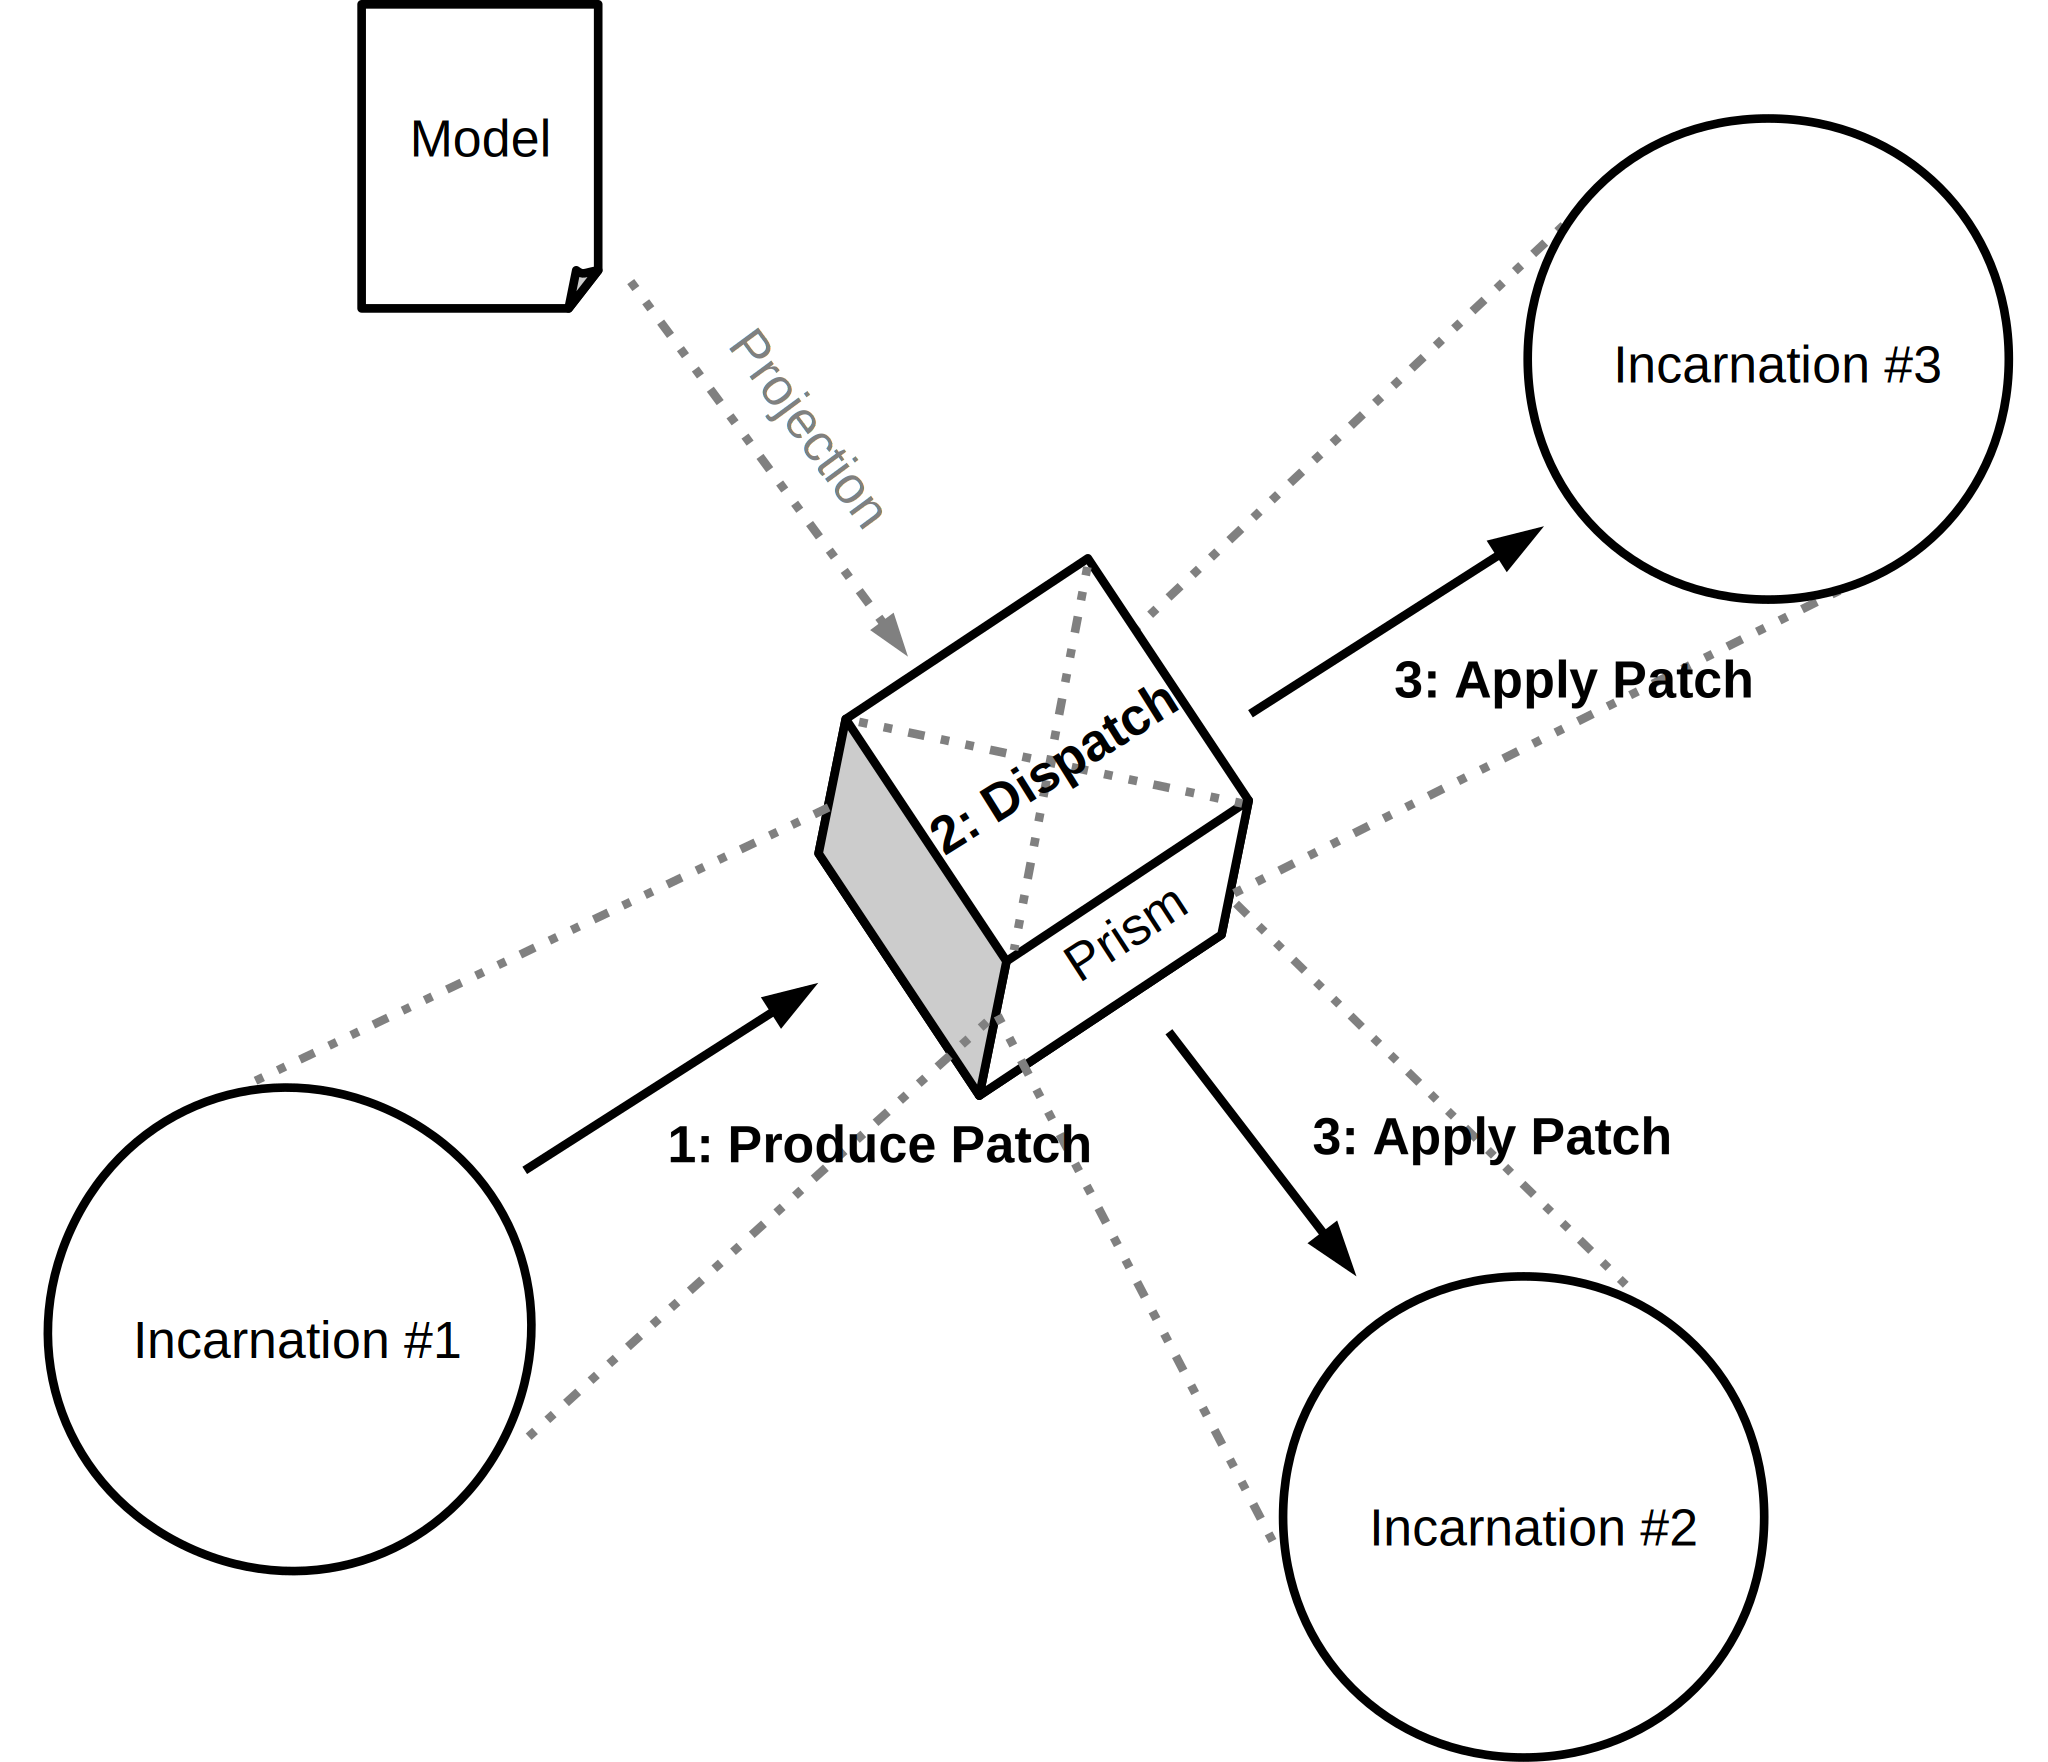
\includegraphics[width=.6\columnwidth]{figures/prism}
	\caption{Using \prism to synchronize three incarnations of the same model. Here, a change occurs on Incarnation \#1 and the resulting patch is shipped to Incarnation \#2 and \#3.}
	\label{fig:prism}
\end{figure}


%Representations of the same model in various LVs are kept in memory to enable online synchronization of the same models manipulated by different stakeholders in different shapes.
%When a changes occurs on either incarnation, the hosting LV is responsible for generating the corresponding \emph{patch}.
%The communication bus then ships this patch to all the other LVs that hold an alternative incarnation of this model.
% (aka. \de or edit script~\cite{rozen2017towards}), that stores the changes on the model that have been realized on this LV.

Every LV then interprets the patch in its own way to keep the representation synchronized.
In EMF, for instance, the patch is interpreted as a set of changes that impact a model conforming to an Ecore metamodel, while in Rascal it is interpreted as a set of changes that impact an ADT value.

As mentioned earlier, each LV may want to preserve extra shape-specific information across the patches.
A textual editor in Rascal, for instance, needs to keep some of the parsing information to maintain layout whenever patches are applied.
So it should be possible to apply the patch while maintaining the extra information specific to a given LV.
Intuitively, our approach supposes that all the information that does not directly relate to the constructs of a language is ``extra'' and therefore should not be part of the patch itself.
There might be cases where sharing extra-information from one shape to the other is desirable, for instance to share layout information between two textual editors.
We discuss this point further in \Cref{sec:discussion}.
%Automatically generating language implementations in different LV is beyond the scope of this paper.
%Instead, given various shapes of a language, implemented by hand, we provide the means to automatically synchronize the projections of a model.

New LVs can be connected to \prism by implementing a simple interface that consists of two operations, namely (i) \emph{produce} which creates a patch materializing the changes on an incarnation and notifies \prism, and (ii) \emph{apply} which receives a patch from \prism and interprets it to update an incarnation, taking into account the specificities of the LV.
The way changes are detected in an incarnation and patches are produced is not prescribed by our approach.
For instance, our Rascal implementation computes patches from a \emph{diff} operation between two ADT values, while our EMF implementation captures the result of transactions on an Ecore model to produce the patches.
The produce and apply operations are implemented once for every LV and do not have to be re-implemented for every language.
%Connecting a LV to \prism consist of producing and interpreting patches for a language.
%A LV has the task of watching changes happening on a incarnation of a model conform to a targeted language and notifying \prism.
%The LV describes the changes in a patch. The patch is an edit script where each operation follows the CRUD-like patch definition.
%After the production of the patch the LV has to notify the \prism.
%In the opposite way a LV can be notified by a patch from the \prism that a change occurred in the model.
%The LV has to interpret this notifying patch to update its own incarnation of the model.
%The interpretation follows the edit script and for each operation applies a change on the incarnation of the model.

A cornerstone artifact in \prism is the dispatch mechanism that routes patches to the appropriate incarnations.
%\prism connects LVs and provides a dispatch mechanism to exchange patches between incarnations of a same model.
When receiving a patch, \prism looks up its internal matrix to determine which other incarnations of the same model should be updated.
%at the corresponding model to find other incarnations of the same model.
The patch is then copied and routed accordingly.
%The lookup is implemented by a matrix internal to \prism linking models to their incarnations. This matrix is kept updated by connected LVs declaring which incarnations of which model they manage.
%\prism addresses the synchronization of different incarnations of same models that is a complementary problem of the collaborative edition.
Our current implementation of the dispatch mechanism is kept simple, and we leave for future work the support of concurrent edits on different incarnations of the same model. This would scale \prism to advanced scenarios that go beyond the scope of this paper, such as collaborative editing.
%Our approach only deals with sequential edition of incarnations and thus complementary work on concurrency in our dispatch mechanism could allow collaborative edition scenarios.

%\td{Highlight incrementality, \ie~we're not Xtext, $\neq$ full de-/re-serialization}

\begin{lstlisting}[label=lst:delta-adt, caption={CRUD-like patch definition in Rascal.}, language=Rascal, float=tb]
@doc{A patch consists of a sequence of edits}
alias Patch = tuple[Id root, Edits edits];

@doc{Edits are operations attached to object identities}
alias Edits = lrel[Id obj, Edit edit];

data Edit
  = put(str field, value val)
  | unset(str field)
  | ins(str field, int pos, value val)
  | del(str field, int pos)
  | create(str class) 
  | destroy();
\end{lstlisting}
